\documentclass[UTF8]{ctexart}
\usepackage{xeCJK}
\setCJKmainfont[BoldFont=Noto Sans S Chinese Bold Bold]{Noto Sans S Chinese Regular}
\usepackage{amsmath}
\usepackage{amsfonts}
\usepackage{geometry}
\geometry{a4paper, left=2cm, right=2cm,top=2cm,bottom=2cm}
\usepackage{pifont}
\usepackage{graphicx}
%\ding{172}=\textcircled{1}
\usepackage{chngcntr}
\usepackage{hyperref}
\counterwithin{equation}{section}
\newcommand{\firstsection}{\subsection}
\newcommand{\secsection}{\subsubsection}
\newcommand{\backdoc}{\normalsize}
\newcommand{\dif}{\mathrm{d}}

\title{Part 3 Statistical Mechanics}
\author{Xiao Liang}
\date{\today}

\begin{document}
	\maketitle
	\tableofcontents
	\newpage
	\CJKfontspec[BoldFont=Noto Sans S Chinese Bold Bold]{Noto Sans S Chinese Regular}
	\section{系综理论初步}
	\firstsection{相空间和刘维尔定理}
	
	\backdoc
	当粒子间的相互作用不能忽略时,应该把系统当做一个整体考虑。先考虑经典描述。假设一个系统由N个\textbf{全同粒子}组成,粒子的自由度为r,则系统的自由度为f=Nr。同理可推广到多粒子的情况。
	
	根据经典力学,系统在任一时刻的微观运动状态由$ f $个广义坐标$ q{_1},q{_2},q{_3},...,q{_f} $及与其共轭的$ f $个广义动量共$ 2f $个变量为直角坐标构成一个$ 2f $维空间,称为\textbf{相空间}。相空间的一个点可以代表系统在某一时刻的运动状态,这个点也被称为系统运动状态的\textbf{代表点}。
	
	系统的运动状态随时间而变,遵从哈密顿正则方程:
	\begin{equation}
	\dot{q}_{i}=\frac{\partial H}{\partial p_{i}}, \quad \dot{p}_{i}=-\frac{\partial H}{\partial q_{i}}, \quad i=1,2, \cdots, r\label{1.1}
	\end{equation}
	
	其中$ H $是系统的哈密顿量,对于保守系统就是能量,包括粒子的动能、粒子相互作用的势能和粒子在保守外场中的势能。它是有关坐标和动量的函数,当存在外场时还是外场参量的函数,但不是时间t的显函数,即:
	
	\begin{equation}
		\frac{\partial H}{\partial t}=0	
	\end{equation}
	
	当系统的运动状态随时间变化时,代表点相应地在相空间中移动,其轨道由式\ref{1.1}决定。考虑到轨道的运动方向完全由$ \dot{q}_{i} $和$ \dot{p}_{i} $确定而哈密顿量和它的微商又都是单值函数,所以经过相空间任意一点的轨道只能有一条,即相空间的运动轨迹是唯一确定的。
		
	由于孤立系统的能量$ E $不随时间而改变,系统的广义坐标和动量必然满足条件:
	\begin{equation}
	H=H\left(q_{1}, \cdots, q_{r} ; p_{1}, \cdots, p_{r}\right)=E\label{1.4}
	\end{equation}
	
	式\ref{1.4}确定了相空间的一个曲面,称为\textbf{能量曲面}。保守系统运动状态的代表点一定位于能量曲面之上。
	
	设想大量结构完全相同的系统,各自从其初态出发独立的沿着正则方程的轨道运动(这种情况下等效于一个系统经历了足够长时间后的结果)。这些系统的运动状态的代表点将在相空间中形成一个分布。相空间中的一个体积元可以表示为:
	\begin{equation}
	\dif  \Omega=\dif  q_{1} \cdots \dif  q_{r} \dif  p_{1} \cdots \dif  p_{r}\tag{1.5}
	\end{equation}
	
	在时间t,运动状态在$ \dif  \Omega $的代表点数为:
	\begin{equation}
	\rho\left(q_{i} ; p_{i} ; t\right) \dif  \Omega\label{1.6}
	\end{equation}
	
	将式\ref{1.6}对整个相空间积分,可得:
	\begin{equation}
	\int \rho\left(q_{i} ; p_{i} ; t\right) \dif  \Omega=N
	\end{equation}
	
	$ N $是所设想的系统的总数,是不随时间改变的常量。
	现在考虑代表点密度$ \rho $随时间t的变化。当时间增加$ \dif t $后,在后一处的密度是:
	
	其中:
	\begin{equation}
	\frac{\dif  \rho}{\dif  t}=\partial_{t} \rho+\sum_{i}\left(\dot{q}_{i} \partial_{q_{i}} \rho+\dot{p}_{i} \partial_{p_{i}} \rho\right)
	\end{equation}
	
	现在要证明:
	\begin{equation}
		\frac{\dif \rho}{\dif t}=0\label{1.10}
	\end{equation}
	
	经过$ \dif t $时间后,该体积元$ \dif  \Omega $中增加的代表点数为$ \frac{\partial \rho}{\partial t} \dif t \dif  \Omega $。这时对六对平面计算净流入体积元的代表点,并由代表点数量守恒的前提得到:
		\begin{equation}
		\frac{\partial \rho}{\partial t} \dif t \dif  \Omega=-\sum_{i}\left[\partial_{q_{i}}\left(\rho \dot{q}_{i}\right)+\partial_{p_{i}}\left(\rho \dot{p}_{i}\right)\right] \dif t \dif  \Omega
		\end{equation}

	结合正则方程(\ref{1.1})可得:
	\begin{equation}
		\partial_{t} \rho+\sum_{i}\left(\dot{q}_{i} \partial_{q_{i}} \rho+\dot{p}_{i} \partial_{p_{i}} \rho\right)=0 \label{1.12}
	\end{equation}
	
	
\noindent 因而证得式\ref{1.10}。这个结论被称为\textbf{刘维尔定理},表明沿着正则方程运动的代表点领域的代表点密度是不随时间改变的常数。
	
	将正则方程(\ref{1.1})代入式\ref{1.12}可得:
	\begin{equation}
	\partial_{t} \rho=-\sum_{i}\left(\frac{\partial \rho}{\partial q_{i}} \frac{\partial H}{\partial p_{i}}-\frac{\partial \rho}{\partial p_{i}} \frac{\partial H}{\partial q_{i}}\right)
	\end{equation}
	
	
\noindent 这是刘维尔定理的另一数学表示。
	
	\section{微正则系综}
	微正则系综是大量这样的系统的集合:系统有固定的能量、粒子数和体积,处于与外界隔绝的状态。
	
	经典力学求解热问题是对每一个粒子进行动力学分析,求出轨迹,然而在热力学需要研究的问题中,这种方法十分繁琐,也很没有必要。原因如下:1、许多感兴趣的系统包含了太多的例子,无法求出它们的轨迹;2、大多数感兴趣的系统都表现出混沌运动,其中时间演化对初始条件的敏感度越来越高——你无法充分了解当前状态来预测未来;3、即使有可能进化出我们的轨迹,知道解决方案在大多数情况下是无用的;比如说,我们更感兴趣的是撞击盒子壁的原子的典型数量,而不是某个特定粒子撞击的精确时间。
	
	在这种情况下,我们转换思路,考虑用一些守恒量作为已知量,并且在且只在了解它们的情况下推导出我们感兴趣的系统的所有状态量。我们先只考虑一个重要的守恒量:系统的能量E,并通过它得到其他的状态量(严格上说V和N也是已知的),这个模型即是微正则系综。
	
	我们计算系统的平均状态在一个长条中:$(E, E+\delta E)$,并令$\delta E \rightarrow 0$。我们定义函数$\Omega(E)$为相空间的体积与$\delta E$的比值,即:
	\begin{equation}
	\Omega(E) \delta E=\int_{E<\mathcal{H}(\mathbb{P}, \mathbb{Q})<E+\delta E} \mathrm{d} \mathbb{P} \mathrm{d} \mathbb{Q}
	\end{equation}
	
	\noindent 这里,$\mathcal{H}(\mathrm{P}, \mathrm{Q})$是系统的哈密顿量,在保守系中可以视为系统的能量。在正则系综中,物理量$\langle O\rangle_{E}$的平均值如下:
	\begin{equation}
	\langle O\rangle_{E}=\frac{1}{\Omega(E) \delta E} \int_{E<\mathcal{H}(\mathbb{P}, 0)<E+\delta E} O(\mathbb{P}, \mathbb{Q}) \dif \mathbb{P} \mathrm{d} \mathbb{Q}
	\end{equation}
	
	接下来作为例子,考虑理想气体。
	
	\firstsection{理想气体}
	
	\secsection{位形空间}
	
	\backdoc
	由于理想气体的运动方程与位置无关,所以其分布在空间中应该是均匀分布。考虑$N$粒子下的体积为$V$的系统,可以得到态密度分布为:
	\begin{equation}
	\rho(\mathbb{Q})=\frac{1}{V^{N}}
	\end{equation}
	
	通过态密度分布和排列问题得到位形概率分布函数:
	\begin{equation}
	P_{m}=2^{-2 N} \left( \begin{array}{c}{2 N} \\ {N+m}\end{array}\right)=2^{-2 N} \frac{(2 N) !}{(N+m) !(N-m) !}
	\end{equation}
	
	考虑斯特林公式:
	\begin{equation}
	n ! \sim(n / \mathrm{e})^{n} \sqrt{2 \pi n} \sim(n / \mathrm{e})^{n}
	\end{equation}
	
	可以得到:
	\begin{equation}
	\begin{aligned}
	P_{m} &\approx 2^{-2 N}\left(\frac{2 N}{\mathrm{e}}\right)^{2 N} /\left(\frac{N+m}{\mathrm{e}}\right)^{N+m}\left(\frac{N-m}{\mathrm{e}}\right)^{N-m}\\
	&=\left(1-m^{2} / N^{2}\right)^{-N}(1+m / N)^{-m}(1-m / N)^{m}
	\end{aligned}
	\end{equation}
	
	\noindent 考虑到在$|m| \ll N$时我们有$1+\epsilon \approx \exp (\epsilon)$,所以:
	\begin{equation}
	P_{m} \approx\left(\mathrm{e}^{-\mathrm{m}^{2} / N^{2}}\right)^{-N}\left(\mathrm{e}^{m / N}\right)^{-m}\left(\mathrm{e}^{-m / N}\right)^{m} \approx P_{0} \exp \left(-m^{2} / N\right)
	\end{equation}
	\noindent 其中,$P_{0}$是一个常数,来源于我们忽略的斯特林公式中的常数。通过归一化积分我们可以得到:
	\begin{equation}
	P_{m} \approx \sqrt{\frac{1}{\pi N}} \exp \left(-\frac{m^{2}}{N}\right)
	\end{equation}
	
	对于宏观系统的许多性质,关于平均值的统计力学波动非常小。
	
	\secsection{动量空间}
	
	\backdoc
	容易想象,在动量空间中的分布是位于一个半径$R=\sqrt{2 m E}$的多维球中。根据一些数学知识可以得到多维球的体积公式:
	\begin{equation}
	\mu\left(\mathbb{S}_{R}^{\ell-1}\right)=\pi^{\ell / 2} R^{\ell} /(\ell / 2) !\label{2.1}
	\end{equation}
	
	通过公式\ref{2.1}可以得到:
	\begin{equation}
	\begin{aligned}
	\frac{\text { shell volume }}{\delta E}&=\frac{\mu\left(S_{\sqrt{2 m(E+\delta E)}}^{3 N-1}\right)-\mu\left(S_{\sqrt{2 m E}}^{3 N-1}\right)}{\delta E}\\
	&=(3 N m) \pi^{3 N / 2} R^{3 N-2} /(3 N / 2) !
	\end{aligned}
	\end{equation}
	
	
	由于在微正则系综模型中,所有状态的权重都相等,所以体积的倒数便可以视为状态出现的概率。现在考虑一个方向上的动量$\rho(p_{1})$,于是半径范围是$(R=\sqrt{2 m E},R^{\prime}=\sqrt{2 m E-p_{1}^{2}})$,由此求出体积和$\delta E$的比值为:
	\begin{equation}
	\begin{aligned}
	\frac{\text { annular area }}{\delta E}&=\mathrm{d} \mu\left(\mathrm{S}^{3 N-2}\right) / \mathrm{d} E\\
	&=(3 N-1) m \pi^{(3 N-1) / 2} R^{\prime 3 N-3} /[(3 N-1) / 2] !
	\end{aligned}
	\end{equation}
	
	最后得到:
	\begin{equation}
		\rho(p_{1})=\left(R^{2} / R^{\prime 3}\right)\left(1-p_{1}^{2} / 2 m E\right)^{3 N / 2}
	\end{equation}
	
	\noindent 考虑到$R^{2} / R^{\prime 3} \approx 1 / R=1 / \sqrt{2 m E}$和$1-p_{1}^{2} / 2 m E=1-\epsilon \approx\exp (-\epsilon)=\exp \left(-p_{1}^{2} / 2 m E\right)$我们可以得到:
	\begin{equation}
	\rho\left(p_{1}\right) \propto \frac{1}{\sqrt{2 m E}} \exp \left(\frac{-p_{1}^{2}}{2 m} \frac{3 N}{2 E}\right)
	\end{equation}
	
	归一化积分后可以得到:
	\begin{equation}
	\rho\left(p_{1}\right)=\frac{1}{\sqrt{2 \pi m(2 E / 3 N)}} \exp \left(\frac{-p_{1}^{2}}{2 m} \frac{3 N}{2 E}\right)
	\end{equation}
	
	考虑到$k_{B} T=2 E / 3 N$(注:现在考虑的都是经典条件下),所以:
	\begin{equation}
	\rho\left(p_{1}\right)=\frac{1}{\sqrt{2 \pi m k_{B} T}} \exp \left(-\frac{p_{1}^{2}}{2 m k_{B} T}\right)\label{equ_micro_rho}
	\end{equation}
	
	从式\ref{equ_micro_rho}可以得到以下几条重要信息:
	
	
	(1)\ 温度。温度可以通过能量和粒子数定义,并且通过式\ref{equ_micro_rho}可以得到相对应的概率密度。
	
	
	(2)\ 玻尔兹曼分布。由式\ref{equ_micro_rho}可以看到对于$ K=\frac{p_{1}^{2}}{2 m} $,概率密度正比于$ e^{-\frac{K}{k_{B}T}} $
	
	
	(3)\ 能均分定理。通过积分可知平均动能$ \left\langle \frac{p_{1}^{2}}{2 m}\right \rangle $的贡献为$ \frac{k_{B} T}{2} $
	
	\subsection{一般情况}
	现在考虑一般情况下的热力学量。首先考虑温度。考虑两个状态$ (s_{1},s_{2})\ and\ E=E_{1}+E_{2} $,可以得到
	\begin{equation}
		\rho\left(s_{1}\right) \propto \Omega_{2}\left(E-E_{1}\right)
	\end{equation}
	
\noindent 由于$ E=E_{1}+E_{2} $,可以得到
\begin{equation}
\Omega(E)=\int \mathrm{d} E_{1} \Omega_{1}\left(E_{1}\right) \Omega_{2}\left(E-E_{1}\right)
\end{equation}

\noindent 由此根据概率密度定义可以得到
\begin{equation}
\rho\left(E_{1}\right)=\Omega_{1}\left(E_{1}\right) \Omega_{2}\left(E-E_{1}\right) / \Omega(E)
\end{equation}

\noindent 考虑等概率原理,达到平衡时应该是系统处于最大概率的时候,这时
\begin{equation}
	\frac{\mathrm{d} \left[\Omega_{1}\left(E_{1}\right) \Omega_{2}\left(E-E_{1}\right)\right]}{\mathrm{d} E_{1}}=0
\end{equation}

\noindent 从而得到
\begin{equation}
\frac{1}{\Omega_{1}}\left.\frac{\mathrm{d} \Omega_{1}}{\mathrm{d} E_{1}}\right|_{E_{m}}=\frac{1}{\Omega_{2}}\left.\frac{\mathrm{d} \Omega_{2}}{\mathrm{d} E_{2}}\right|_{E-E_{m}}\label{equ_micro_Omega}
\end{equation}

	通过这个式子可以定义温度。考虑到更多时候我们使用的是$ \ln \Omega $,定义
	\begin{equation}
		S(E)=k_{B} \ln \left(\Omega(E)\right)\label{equ_micro_S}
	\end{equation}
	
	为系统的\textbf{熵},熵也因此成为微正则系综的配分函数。通过熵可以得到所有的热力学量,当然包括它自己。这个关系是著名的\textbf{玻尔兹曼关系},在现在的推导之下,它不仅适用于之前的近独立粒子系统,也可以适用于包含相互作用的微正则系统,同时,考虑对非平衡状态的系统,将系统分为若干个彼此微弱作用又处在局域平衡的部分,由于熵具有可加性,微观态数为简单的连乘关系,可推知玻尔兹曼关系在非平衡状态下也是成立的。这是统计力学优越的地方所在。
	
	考虑到$ \frac{\dif S}{\dif E} =\frac{k_{B}}{\Omega} \frac{\dif \Omega}{\dif E} $,代入式\ref{equ_micro_Omega}可得:
	\begin{equation}
	\frac{\mathrm{d}}{\mathrm{d} E_{1}}\left(S_{1}\left(E_{1}\right)+S_{2}\left(E-E_{1}\right)\right)=\left.\frac{\mathrm{d} S_{1}}{\mathrm{d} E_{1}}\right|_{E_{m}}-\left.\frac{\mathrm{d} S_{2}}{\mathrm{d} E_{2}}\right|_{E-E_{m}}=0
	\end{equation}
	
	
\noindent 这等价于$ \frac{\dif \left(S_{1}+S_{2}\right)}{\dif E_{1}}=0 $,所以
\begin{equation}
\frac{\mathrm{d} S_{1}}{\mathrm{d} E_{1}}=\frac{\mathrm{d} S_{2}}{\mathrm{d} E_{2}}
\end{equation}

\noindent 由此定义温度:
\begin{equation}
	\left.\frac{1}{T}=\frac{\partial S}{\partial E}\right|_{V,E}
\end{equation}

	可将熵$ S $视为$ E,V,N $的函数,则根据热力学关系可得:
	\begin{equation}
	\begin{aligned}
	\frac{P}{T}&=\left.\frac{\partial S}{\partial V}\right|_{E, N}\\
	-\frac{\mu}{T}&=\left.\frac{\partial S}{\partial N}\right|_{E, V}
	\end{aligned}
	\end{equation}
	
	根据偏导关系可得压强和化学势的定义:
	\begin{equation}
	\begin{aligned}
		\left.\frac{\partial E}{\partial V}\right|_{S, N}&=-P\\
		\left.\frac{\partial E}{\partial N}\right|_{S, V}&=\mu
	\end{aligned}
	\end{equation}
	
	结合之前的理想气体的微观态表达式,可以推出所有的热力学量,此处不赘述。
	
	\section{正则系综}
	正则系统是更为实际的系统,其具有确定的粒子数、体积和温度。这样的系统可以设想为与大热源接触并达到平衡的系统。两者可以交换能量,因此系统可能的微观状态可具备不同的能量值。在两者建立平衡之后,系统将与热源具有相同的温度。
	
	\subsection{一般情况}
	系统和热源结合起来成为一个复合系统,由于这个复合系统能量恒定,可以认为是一个微正则系综。假设系统的能量为$ \varepsilon $,所以$ E=\varepsilon+E_{h} $。当将系统和热源作为整体考虑时可以知道,系统在某个能量下的微观数就是热源在其共轭能量下的微观数,考虑概率密度同微观状态数的关系,可以得到
	\begin{equation}
		P(\varepsilon) \approx \Omega(E-\varepsilon)
	\end{equation}
	
	由于$ \varepsilon \ll E $,可以对$ \ln \Omega(E-\varepsilon) $在$ \varepsilon=0 $处进行泰勒展开(其实就是将$ \varepsilon $视为微小量),并忽略高阶项,由此得:
	\begin{equation}
		\ln \Omega(E-\varepsilon)= \ln \Omega(E)-\frac{\varepsilon}{k_{B} T}
	\end{equation}
	
\noindent 可以证明,第二项开始的贡献都小到可以忽略不计。

	由此可以得到:
	\begin{equation}
		P(\varepsilon) \approx e^{-\frac{\varepsilon}{k_{B} T}}
	\end{equation}
	
\noindent 这个分布称为\textbf{玻尔兹曼分布},也称\textbf{正则分布},因子$ e^{-\frac{\varepsilon}{k_{B} T}} $被称为\textbf{玻尔兹曼因子}。对其进行归一化,分母的和式$ \sum_{i}  e^{-\frac{E_{i}}{k_{B} T}}$即是正则配分函数。(注意,此处没有考虑简并度,所以和式中存在大量的相同量)
		
		通过配分函数可以得到以下热力学量:
		\begin{equation}
		\begin{aligned}
			U&=\overline{E}=-\frac{\partial}{\partial \beta} \ln Z\\
			Y&=\overline{\frac{\partial E}{\partial y}}=- \frac{1}{\beta} \frac{\partial}{\partial y} \ln Z\\
			S&=k_{B} \left(\ln Z-\beta \frac{\partial}{\partial \beta} \ln Z\right)\\
			F&=-k \ln Z
		\end{aligned}
		\end{equation}
		
	\noindent 由此可见,正则系综的特性函数是$ F(N,V,T) $
	
	定义能量涨落为$ \overline{\left(E-\overline{E}\right)^{2}} $,故:
	\begin{equation}
		\overline{\left(E-\overline{E}\right)^{2}}=\overline{E^{2}}-\left(\overline{E}\right)^{2}
	\end{equation}

\noindent 对于正则分布
\begin{equation}
	\frac{\partial \overline{E}}{\partial \beta}= -\left[\overline{E^{2}}-\left(\overline{E}\right)^{2}\right]
\end{equation}

\noindent 所以
\begin{equation}
	\overline{\left(E-\overline{E}\right)^{2}}=k T^{2} C_{V}
\end{equation}

\noindent 由此可以看出,在稳定条件下,$ C_{V} $必然为正。可以证明,对于一个和热源接触达到平衡的系统,虽然会因为与热源交换能量而具有不同的能量值,但对于宏观的系统,$ E $与$ \overline{E} $有显著偏差的概率是极小的。这个事实告诉我们,用微正则分布和正则分布求得的热力学量是相同的,实质上只相当于选取不同的特性函数。

	\subsection{实际气体的物态方程}
	在低密度下可以将气体视为理想气体,但在高密度下气体分子间的相互作用不可忽略,此时理想气体模型不再使用。系统理论可以处理互作用粒子组成的系统(虽然还是比较麻烦)。
	
	考虑单原子分子的经典气体。设气体含有$ N $个分子,气体的能量为
	\begin{equation}
		E= \sum_{i=1}^{N} \frac{p_{i}^{2}}{2m} + \sum_{i<j} \Phi \left(r_{ij}\right)
	\end{equation}
	
\noindent 假设粒子间的相互作用能量$ \Phi \left(r_{ij}\right) $只跟分子间距有关,由于每一对分子的互作用能量在求和中都出现且只出现一次,故共包括$ \frac{1}{2} N(N-1) $项。由于$ N $很大,可以认为有$ \frac{1}{2} N^{2} $

 	由正则分布求物态方程,需要求配分函数$ Z $:
 	\begin{equation}
 	Z=\frac{1}{N! h^{3N}} \int \cdots \int e^{-\beta E} \dif q_{1} \cdots \dif q_{3N} \dif p_{1} \cdots \dif p_{3N}
 	\end{equation}

\noindent 式中,含动量的配分函数可以分离变量,这样可以先求出动量部分的积分,为
\begin{equation}
	\prod_{i=1}^{3N} \int_{-\infty}^{\infty} e^{-\beta \frac{p_{i}^{2}}{2m}}  \dif p_{i}= \left(\frac{2 \pi m}{\beta}\right)^{\frac{3 N}{2}}
\end{equation}

	配分函数的第二部分定义为$ Q=\int \cdots \int e^{\beta \sum_{i<j} \Phi \left(r_{ij}\right)} \dif q_{1} \cdots \dif q_{N} $,被称为\textbf{位形积分}。这个积分由于每一项都有两个分子的坐标,而每个分子的坐标都出现在乘积的$ N-1 $项,在数学上十分的复杂。
	
	定义函数
	\begin{equation}
		f_{ij} = e^{\beta \Phi \left(r_{ij}\right)}-1
	\end{equation}
	
\noindent 当$ r_{ij} $大于分子的相互作用力程时,势能项为零,使得$ f_{ij} $为零。分子的相互作用力是短程力,力程约为分子直径的三四倍,因此$ f_{ij} $仅在极小的空间范围内不等于零。利用$ f_{ij} $可将位形积分表示为
\begin{equation}
Q=\int d^{3 N} q\left(1+\sum_{i<j} f_{i j}+\sum_{i<j} \sum_{i^{\prime}<j^{\prime}} f_{i j} f_{i^{\prime} j^{\prime}}+\cdots\right)\label{equ_Q}
\end{equation}

\noindent 如果上式只保留第一项,相当于理想气体近似。对于后面几项的物理图像如下:
\begin{figure}[ht]
	\centering
	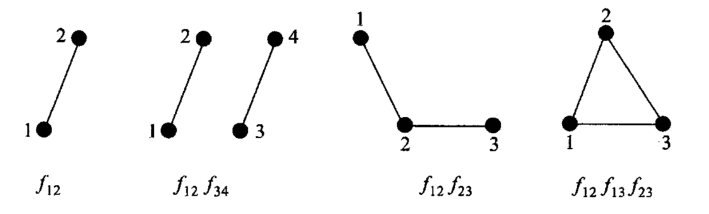
\includegraphics[width=12cm]{static_pratical_gas.png}
	\caption{\ref{equ_Q}式后几项的图像表示}
	\label{figure_practical_gas}
\end{figure}

	在只考虑二阶位力系数的情况下,我们得到:
	\begin{equation}
	Q=\int d^{3 N} q\left(1+\sum_{i<j} f_{i j}\right)
	\end{equation}
	
	对于括号里的第二项,每一项都可以得到:
	\begin{equation}
		F=V^{N-2} \int \int f_{12} \dif q^{1} \dif q^{2}
	\end{equation}
	
\noindent 略去边界效应,积分可以化为:
\begin{equation}
	\int f_{12} \dif q^{1} \dif q^{2} = V \int f_{12} \dif \mathbf{r}
\end{equation}

\noindent 其中$ \mathbf{r} $是两分子的相对坐标,由此可以得到:
\begin{equation}
	\begin{aligned}
	Q&=V^{N}\left[1+\frac{N^{2}}{2 V} \int d^{3} r f_{12}\right]\\
	Z&=\frac{1}{N !}\left(\frac{2 \pi m}{\beta h^{2}}\right)^{3 N / 2} V^{N}\left[1+\frac{N^{2}}{2 V} \int d^{3} r f_{12}\right]
	\end{aligned}
\end{equation}

	根据压强的关系式$ P=\frac{1}{\beta} \partial_{V} \ln Z $可得
	\begin{equation}
	P V \equiv N k_{B} T\left(1+\frac{n B}{V}\right)
	\end{equation}
	
\noindent 第二位力系数由此可得:
\begin{equation}
B=-\frac{N_{A}}{2} \int d^{3} r f_{12}
\end{equation}

	分子间的相互作用势由半经验的公式$ \phi(r)=\phi_{0} \left[\left(\frac{r_{0}}{r}^{12}\right)-2 \left(\frac{r_{0}}{r}^{6}\right)\right] $给出。为了简化计算,采用较为粗略的近似
	\begin{equation}
	\begin{aligned}
	\phi(r)&=+\infty \quad r<r_{0}\\
	\phi(r)&=-\phi_{0} \left(\frac{r_{0}}{r}\right)^{6} \quad r \geq r_{0}
	\end{aligned}\label{equ_phi}
	\end{equation}
	
	根据上式计算第二位力系数B。用球坐标表示可得:
	\begin{equation}
	B=-\frac{N_{A}}{2} \int d^{3} r f_{12}=-2 \pi N_{A} \int_{0}^{\infty} r^{2} d r\left[e^{-\beta \phi(r)}-1\right]
	\end{equation}
	
\noindent 代入式\ref{equ_phi},得到:
\begin{equation}
B=2 \pi N_{A}\left\{\int_{0}^{r_{0}} r^{2} d r-\int_{r_{0}}^{\infty} r^{2} d r\left[e^{-\beta \phi(r)}-1\right]\right\}
\end{equation}

\noindent 如果气体的温度足够高,分子的平均动能将大于其相互作用势能,即$ \frac{\phi_{0}}{k T} \ll 1 $,由此可得积分:
\begin{equation}
B=2 \pi N_{A}\left(\frac{r_{0}^{3}}{3}-\frac{4 \beta \epsilon r_{0}^{3}}{3}\right)=b-\frac{\beta a}{N_{A}}
\end{equation}

\noindent 由于$ \frac{n b}{V} \ll 1 $,取近似$ 1+\frac{n b}{V}=\frac{1}{\left(1- \frac{n b}{V}\right)} $,可得到著名的\textbf{范德瓦尔斯方程}:
\begin{equation}
\left(P+\frac{n^{2} a}{V^{2}}\right)(V-n b)=NkT
\end{equation}

\noindent 由上述粗略结果得到的$ a,b $是与温度无关的常量,实际气体的$ a,b $值则与温度有关。

	\subsection{固体的热容}
	固体中相邻原子由于存在很强的相互作用,原子在其平衡位置附近作微振动 ,考虑$ N $个原子,设$ q_{i} $表示第$ i $个自由度偏离其平衡位置的位移,相应的动量为$ p_{i} $,势能可以展为$ q_{i} $的幂级数,准确到二级为
	\begin{equation}
	\phi=\phi_{0}+ \sum_{i} \left(\partial_{i} \phi \right)_{0} q_{i} \frac{1}{2} \sum_{i, j}\left(\partial_{i} \partial_{j} \phi\right)_{0} q_{i} q_{j}
	\end{equation}
	
\noindent $ \phi_{0} $是所有原子都位于平衡位置时原子间的相互作用能。而位于平衡位置时可知$ \left(\partial_{i} \phi\right)_{0} q_{i}=0 $,再考虑线性变换使得二次型化为平方和(即寻找一套解耦的广义坐标),可得到
\begin{equation}
E=\phi_{0}+\frac{1}{2} \sum_{i=1}^{3 N}\left(p_{i}^{2}+w_{i}^{2} q_{i}^{2}\right)
\end{equation}

注意,这里的$ q_{i} $是简正坐标,和全体原子的位移都有关,在这套坐标之下复杂的相关运动变成了简正振动。

	根据量子理论,得到能量为
	\begin{equation}
	E_{s}=\phi_{0}+\sum_{i=1}^{3 N} \hbar w_{i}\left(n_{s i}+\frac{1}{2}\right), \quad n_{s i}=0,1,2, \cdots
	\end{equation}
	
\noindent 由此可得到\textbf{系统}的配分函数为
\begin{equation}
	\begin{aligned}
	Z&=e^{-\beta \phi_{0}} \prod_{i=1}^{3 N} \sum_{n_{s i}=0}^{\infty} e^{-\beta \hbar w_{i}\left(n_{s i}+1 / 2\right)}\\
	&=e^{-\beta \phi_{0}} \prod_{i=1}^{3 N} \frac{e^{-\frac{1}{2} \beta \hbar w_{i}}}{1-e^{-\beta \hbar w_{i}}}
	\end{aligned}\label{equ_Z_si}
\end{equation}

\noindent 根据此可得内能
\begin{equation}
	U=-\partial_{\beta} \ln Z=U_{0}+\sum_{i=1}^{3 N} \frac{\hbar w_{i}}{e^{\beta \hbar w_{i}}-1}
\end{equation}

\noindent 其中$U_{0}=\phi_{0}+\sum_{i=1}^{3 N} \frac{\hbar w_{i}}{2}$。分析可得,$ \phi_{0}<0 \ and\ U_{0}<0 $。$ U_{0} $是固体的\textbf{结合能},第二项是热运动能量。

	现在开始需要考虑简正振动的频率分布。如果假设其简正振动的频率都一样的话,便是爱因斯坦模型。德拜将固定看做连续弹性介质,$ 3N $个简正振动是弹性介质的基本波动。固体上传播的弹性波有纵波和横波两种,纵波是膨胀压缩波,横波是扭转波。对一定的波矢,纵波只有一种振动方式,而横波有两种振动方式。
	
	考虑$ \omega=ck $可以得到
	\begin{equation}
		D(w) \dif w=\frac{V}{2 \pi^{2}}\left(\frac{1}{c_{l}^{3}}+\frac{2}{c_{t}^{3}}\right) w^{2} \dif w \equiv B w^{2} \dif w
	\end{equation}
	
\noindent 其中$ B=\frac{V}{2 \pi^{2}} \left(\frac{1}{c_{l}^{3}}+\frac{2}{c_{t}^{3}}\right) $

\noindent 必须假设存在一个最大的圆频率$ \omega_{D} $,令
\begin{equation}
	\int_{0}^{\omega_{D}} B \omega^{2} \dif \omega = 3 N
\end{equation}

\noindent 可得
\begin{equation}
w_{D}^{3}=\frac{9 N}{B}
\end{equation}

\noindent 其中$ \omega_{D} $称为德拜频率。

	令$ x=\frac{\hbar \omega_{D}}{k T}=\frac{\theta_{D}}{T} $,$ \theta_{D} $也被称为德拜特征温度,是物质的特征参量,考虑高温和低温极限$ x \ll 1, x \gg 1 $得到
	\begin{equation}
	\begin{aligned}
	U&=U_{0}+3NkT\\
	C_{V}&=3Nk
	\end{aligned}
	\end{equation}
	
\noindent 和
\begin{equation}
	\begin{aligned}
	U&=U_{0}+3Nk \frac{\pi^{4}}{5} \frac{T^{4}}{\theta_{D}^{3}}\\
	C_{V}&=3nk \frac{4 \pi^{4}}{5} \left(\frac{T}{\theta_{D}}\right)^{3}
	\end{aligned}
\end{equation}

\noindent 低温极限时忽略了自由电子对热熔的贡献,在温度$ T>3K $时是符合的。

	德拜将固体近似看作连续弹性介质,忽略了固体中原子的离散结构,在波长远大于平均距离的简谐振动时,相邻原子在振动中的位移近似相等,德拜近似与实际情况是接近的。
	
	也可以从粒子角度进行研究,将简正振动的能量量子看作一种准粒子,称为\textbf{声子},得到的结果一样。
	
	\section{巨正则系综}
	当系统的各个可能的微观状态中,粒子数和能量均可具有不同的数值时,需要考虑巨正则系综。巨正则分布是具有确定的\textbf{体积、温度和化学势}的系统的分布函数。
	
	\subsection{一般情况}
	仿照正则系综的方式,假设同一个很大的源接触,构成一个复合系统,对于复合系统可以视为微正则系综。经过相同的处理,可得巨正则分布函数
	\begin{equation}
	\rho_{Ns}=\frac{1}{\Xi} e^{-\alpha N-\beta E_s}
	\end{equation}
	
\noindent 其中$ \Xi $为巨配分函数,为
\begin{equation}
	\Xi=\sum_{N=0}^{\infty} \sum_{s} e^{-\alpha N-\beta E_{s}}
\end{equation}

\noindent 其中$ \alpha=-\frac{\mu}{kT}, \beta=\frac{1}{kT} $

	巨正则分布的经典表达式为
	\begin{equation}
		\rho(q, p) \dif \Omega=\frac{1}{N ! h^{N r}} \frac{e^{-\alpha N-\beta E(q, p)}}{\Xi} \dif \Omega
	\end{equation}
	
\noindent 其中巨配分函数为
\begin{equation}
	\Xi= \sum_{N=0} \frac{e^{\alpha N}}{N ! h^{Nr}} \int e^{-\beta E(q,p) \dif \Omega}
\end{equation}

	\subsection{巨正则系综理论的热力学公式}
	由于系统和源可以交换粒子和能量,在系统各个可能的微观状态中,其粒子数和能量值不是确定的。系统的平均粒子数$ \overline{N} $是粒子数对给定条件下一切可能的微观状态的平均值:
	\begin{equation}
	\overline{N}=\frac{1}{\Xi} \sum_{N} \sum_{s} N e^{-\alpha N-\beta E_{s}}=-\partial_{\alpha} \ln \Xi
	\end{equation}
	
\noindent 内能是能量的统计平均值:
\begin{equation}
U=\frac{1}{\Xi} \sum_{N} \sum_{s} E_{s} e^{-\alpha N-\beta E_{s}}=-\partial_{\beta} \ln \Xi
\end{equation}

\noindent 广义力:
\begin{equation}
Y=\frac{1}{\Xi} \sum_{N} \sum_{s} \partial_{y} E_{s} e^{-\alpha N-\beta E_{s}}=-\frac{1}{\beta} \partial_{y} \ln \Xi
\end{equation}

\noindent 求熵向来比较复杂,先考虑
\begin{equation}
\beta\left(\dif U-Y \dif y+\frac{\alpha}{\beta} \dif \overline{N}\right)=\dif \left(\ln \Xi-\alpha \partial_{\alpha} \ln \Xi-\beta \partial_{\beta} \ln \Xi\right)
\end{equation}

\noindent 经过比较
\begin{equation}
\frac{1}{T}(\dif U-Y \dif y-\mu \dif \overline{N})=\dif S
\end{equation}

\noindent 可以得到
\begin{equation}
S=k\left(\ln \Xi-\alpha \partial_{\alpha} \ln \Xi-\beta \partial_{\beta} \ln \Xi\right)
\end{equation}

\noindent 巨热力势
\begin{equation}
J=U-T S-\mu \overline{N}=-k T \ln \Xi
\end{equation}

	现在来考虑粒子数的涨落。首先写出粒子数涨落的表达式
	\begin{equation}
	\overline{\left(N-\overline{N}\right)^{2}}=\overline{N^{2}}-\left(\overline{N}\right)^2
	\end{equation}
	
\noindent 但
\begin{equation}
	\frac{\partial \overline{N}}{\partial \alpha} = -\left[\overline{N^{2}}-\left(\overline{N}\right)^2\right]
\end{equation}

\noindent 所以
\begin{equation}
	\overline{\left(N-\overline{N}\right)^{2}}=-\left(\frac{\partial \overline{N}}{\partial \alpha}\right)_{\beta,y}=kT\left(\frac{\partial \overline{N}}{\partial \mu}\right)_{T,V}
\end{equation}

	\subsection{巨正则系综理论的简单应用}
	\subsubsection{吸附现象}
	
	设吸附表面有$ N_{0} $个吸附中心,每个吸附中心可吸附一个气体分子。被吸附的气体分子能量为$ -\varepsilon_{0} $。求达到平衡时吸附率$ \theta=\frac{N}{N_{0}} $与气体温度和压强的关系。
	
	将气体看作热源和粒子源。被吸附的分子看作可与气体(源)交换粒子和能量的系统,遵从巨正则分布。当有$ N $个分子被吸附时,系统的能量为$ -N\varepsilon_{0} $。考虑$ N $个分子在$ N_{0} $个吸附中心上有$ \frac{N_{0} !}{N! \left(N-N_{0}\right) !} $个不同的排列,系统的巨配分函数为(注意$ \alpha=-\beta \mu $)
	\begin{equation}
	\Xi=\sum_{N=0}^{N_{0}} \sum_{s} e^{-\alpha N-\beta E_{s}}=\sum_{N=0}^{N_{0}} \frac{N_{0} !}{N !\left(N_{0}-N\right) !} e^{\beta\left(\mu+\varepsilon_{0}\right) N}=\left[1+e^{\beta\left(\mu+\varepsilon_{0}\right)}\right]^{N_{0}}
	\end{equation}
	
	达到平衡时,系统(被吸附的分子)与气体的化学势和温度应该相等,所以
	\begin{equation}
		e^{-\alpha}=e^{\beta \mu}=\frac{N \lambda^{3}}{V}
	\end{equation}
	
\noindent 所以
\begin{equation}
	\theta= \frac{\overline{N}}{N_{0}}=\frac{1}{1+\frac{N \lambda^{3}}{V} e^{-\frac{\varepsilon_{0}}{k T}}}
\end{equation}

	\subsubsection{由巨正则系综理论导出近独立粒子的平均分布}
	写出巨正则配分函数
	\begin{equation}
		\Xi =\sum_{N} \sum_{s} e^{-\alpha N-\beta E_{s}}=\prod_{l} \sum_{a_{l}} e^{-\left(\alpha+\beta_{l}\right) a_{l}}
	\end{equation}
	
\noindent 可表述为$ \Xi =\prod_{l} \Xi_{l} $,容易得到
	\begin{equation}
		\overline{a}_{l} = -\frac{\partial}{\partial \alpha} \ln \Xi_{l}
	\end{equation}
	
	对于玻色子,能级$ \varepsilon_{l} $上的粒子数没有限制,在能级配分函数的求和中,$ a_{l} $可以取从0到$ \infty $的任何值,因此得
	\begin{equation}
	\begin{aligned}
	\Xi_{l} &=\frac{1}{1-e^{-\alpha-\beta \varepsilon_{l}}}\\
	\overline{a}_{l}&=-\frac{\partial}{\partial \alpha} \ln \Xi_{l}=\frac{1}{e^{\alpha+\beta \varepsilon_{l}}-1}
	\end{aligned}
	\end{equation}
	
	对于费米子,由于泡利不相容原理的限制,能级$ \varepsilon_{l} $上可能的粒子数为0或1,因此
	\begin{equation}
		\begin{aligned}
		\Xi_{l} &=\sum_{a_{l}=0}^{1} e^{-\left(\alpha+\beta \varepsilon_{l}\right)}=1+e^{-\left(\alpha+\beta \varepsilon_{l}\right)}
		\\
		\overline{a}_{l}&=-\frac{\partial}{\partial \alpha} \ln \Xi_{l} =\frac{1}{e^{\alpha+\beta \varepsilon_{l}}+1}
		\end{aligned}
	\end{equation}
	
	如果能级$ \varepsilon_{l} $有$ \omega_{l} $个量子态,能级$ \varepsilon_{l} $上的平均粒子数应为上述两式的$ \omega_{l} $倍:
	\begin{equation}
		\overline{a}_{l} =\frac{\omega_{l}}{e^{\alpha+\beta \varepsilon_{l}} \pm 1}
	\end{equation}

\noindent 具体证明见书本附录。
\end{document}
